\documentclass{article}

\usepackage{algorithmicx}
\usepackage{algpseudocode}
\usepackage{graphicx}
\usepackage{listings}
\usepackage{amsmath}
\usepackage{textcomp}
\usepackage{color}
\usepackage[%  
    colorlinks=true,
    pdfborder={0 0 0},
    linkcolor=blue
]{hyperref}

\lstset{ %
  language=Java,                  % the language of the code
  basicstyle=\footnotesize,       % the size of the fonts that are used for the code
  numbers=left,                   % where to put the line-numbers
  numberstyle=\tiny\color{gray},  % the style that is used for the line-numbers
  stepnumber=1,                   % the step between two line-numbers. If it's 1, each line
                                  % will be numbered
  numbersep=5pt,                  % how far the line-numbers are from the code
  backgroundcolor=\color{white},  % choose the background color. You must add \usepackage{color}
  showspaces=false,               % show spaces adding particular underscores
  showstringspaces=false,         % underline spaces within strings
  showtabs=false,                 % show tabs within strings adding particular underscores
  frame=single,                   % adds a frame around the code
  rulecolor=\color{black},        % if not set, the frame-color may be changed on line-breaks within not-black text (e.g. commens (green here))
  tabsize=4,                      % sets default tabsize to 2 spaces
  captionpos=b,                   % sets the caption-position to bottom
  breaklines=true,                % sets automatic line breaking
  breakatwhitespace=false,        % sets if automatic breaks should only happen at whitespace
  title=\lstname,                 % show the filename of files included with \lstinputlisting;
                                  % also try caption instead of title
  keywordstyle=\color{blue},          % keyword style
  commentstyle=\color{dkgreen},       % comment style
  stringstyle=\color{mauve},         % string literal style
  escapeinside={\%*}{*)},            % if you want to add a comment within your code
  morekeywords={*,...}               % if you want to add more keywords to the set
}

\newcommand{\comment}[1]{}

\title{Assignment Week 3 - Questions and Solutions}
\author{Course: Building Blocks of Programming}
\date{Topic: Flowcharts - Loops}
\begin{document}
\maketitle

\begin{flushleft}

    \textbf{Q 1. } Draw a flowchart that takes a positive integer “n”  as input and 
    displays the sum of all the positive integers which are less than or equal to n 
    and divisible by 6 but not by 5.
    
    \end{flushleft}
    
    \begin{flushleft}
    
    \textbf{Ans. } We can simply iterate over all numbers and print if the conditions
    are satisfied. Sample flowchart is in Fig \ref{Q1}.
    
    \end{flushleft}
    
    \begin{flushleft}
    
    \textbf{Grading. } If the output of flowchart is correct then 2, if there are 
    errors but the overall intent/logic is correct then 1 otherwise 0.
    
\end{flushleft}
    
    \begin{figure}[ht]
        \centering
        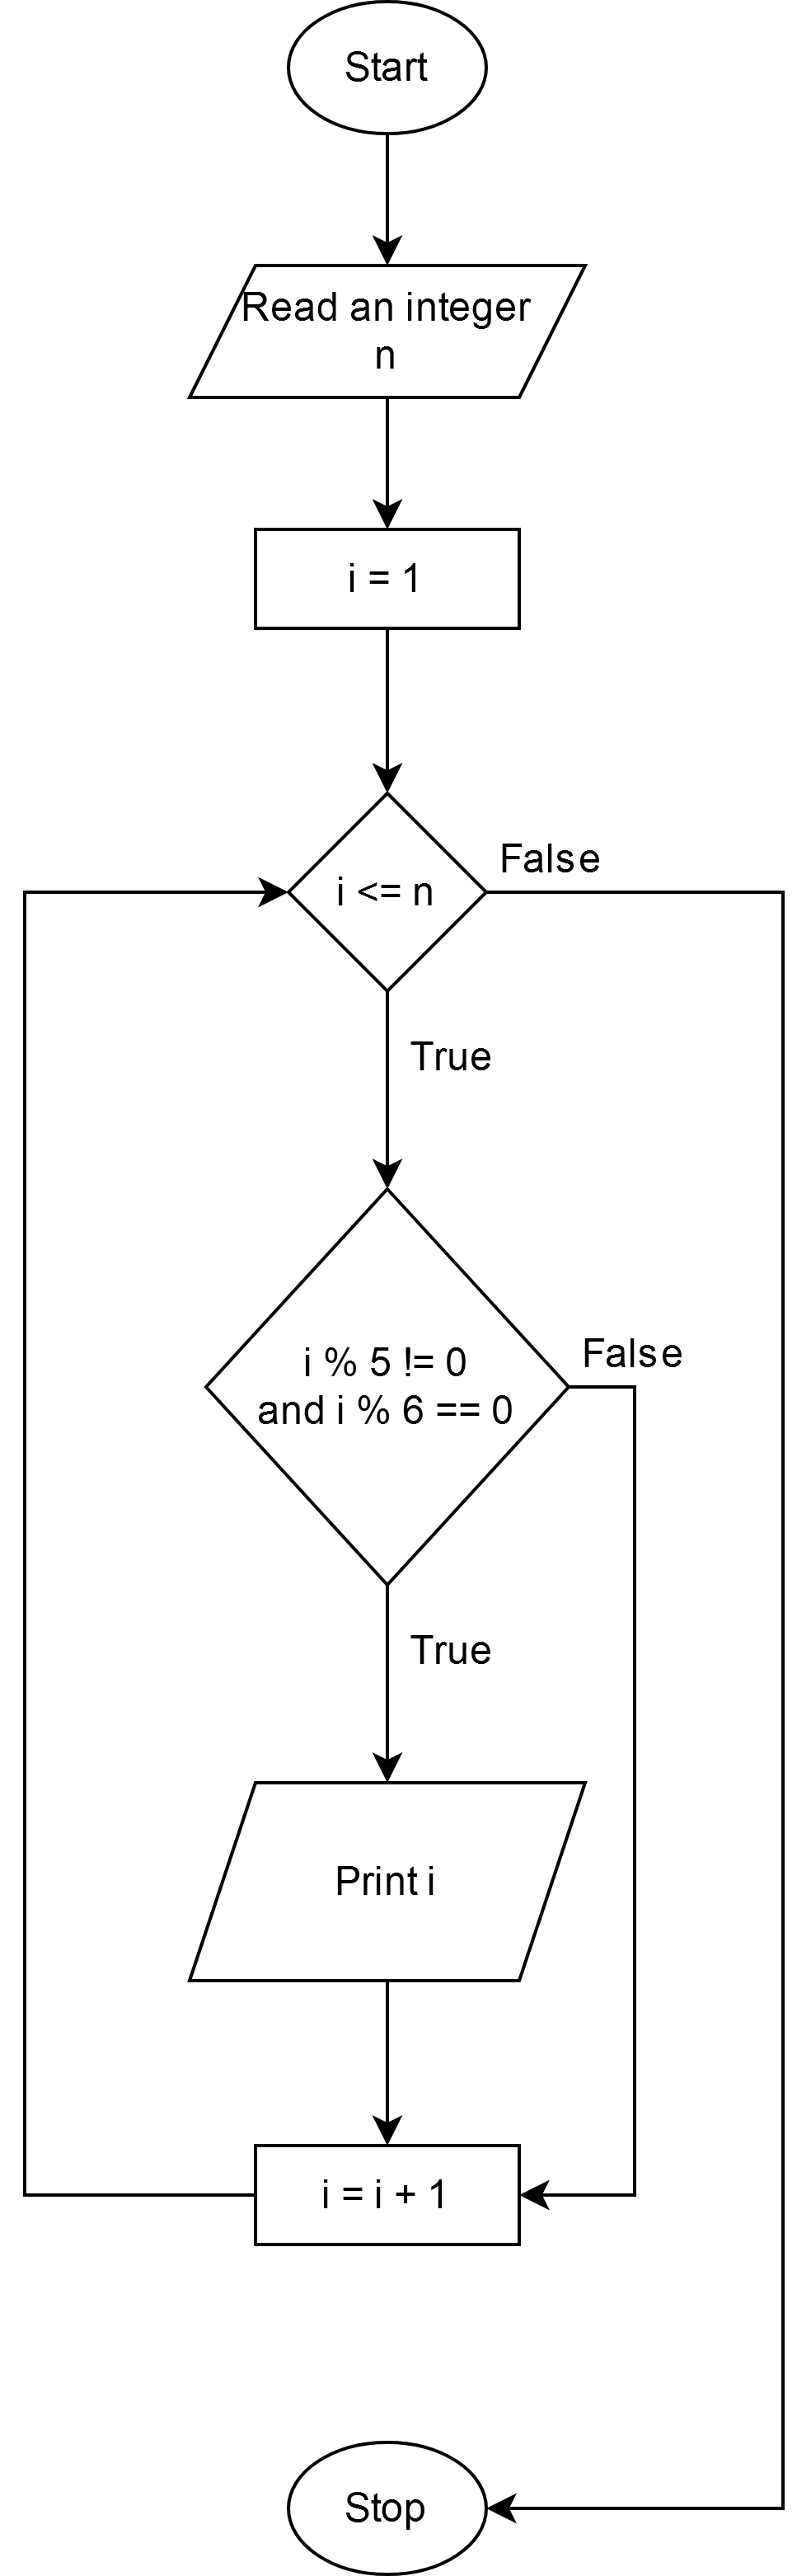
\includegraphics[width=0.35\textwidth]{Q1.png}
        \caption{Sample flowchart for Q1}
        \label{Q1}
    \end{figure}
    
\clearpage


\begin{flushleft}

    \textbf{Q 2. } Draw a flowchart that takes a positive integer as input and 
    print “Yes” if the number is prime otherwise print “No”.

    
    \end{flushleft}
    
    \begin{flushleft}
    
    \textbf{Ans. } We iterate over all the numbers from 2 upto n-1 and print
    "No" if we are able to find a factor, otherwise print "Yes". 
    Sample flowchart is given in Fig \ref{Q2}.
    We use the "\%" operator to check divisibility, i.e. $i$ is factor of $n$
    only if $n \% i == 0$
    We can run it for numbers upto $\frac{n}{2}$ or $\sqrt{n}$ instead of $n-1$
    but such optimisations are not required.
    
    \end{flushleft}
    
    \begin{flushleft}
    
    \textbf{Grading. } If the output is correct then 2, if there are errors in
    the logic but the overall intent is correct then 1, otherwise 0.
    
\end{flushleft}
    
    \begin{figure}[ht]
        \centering
        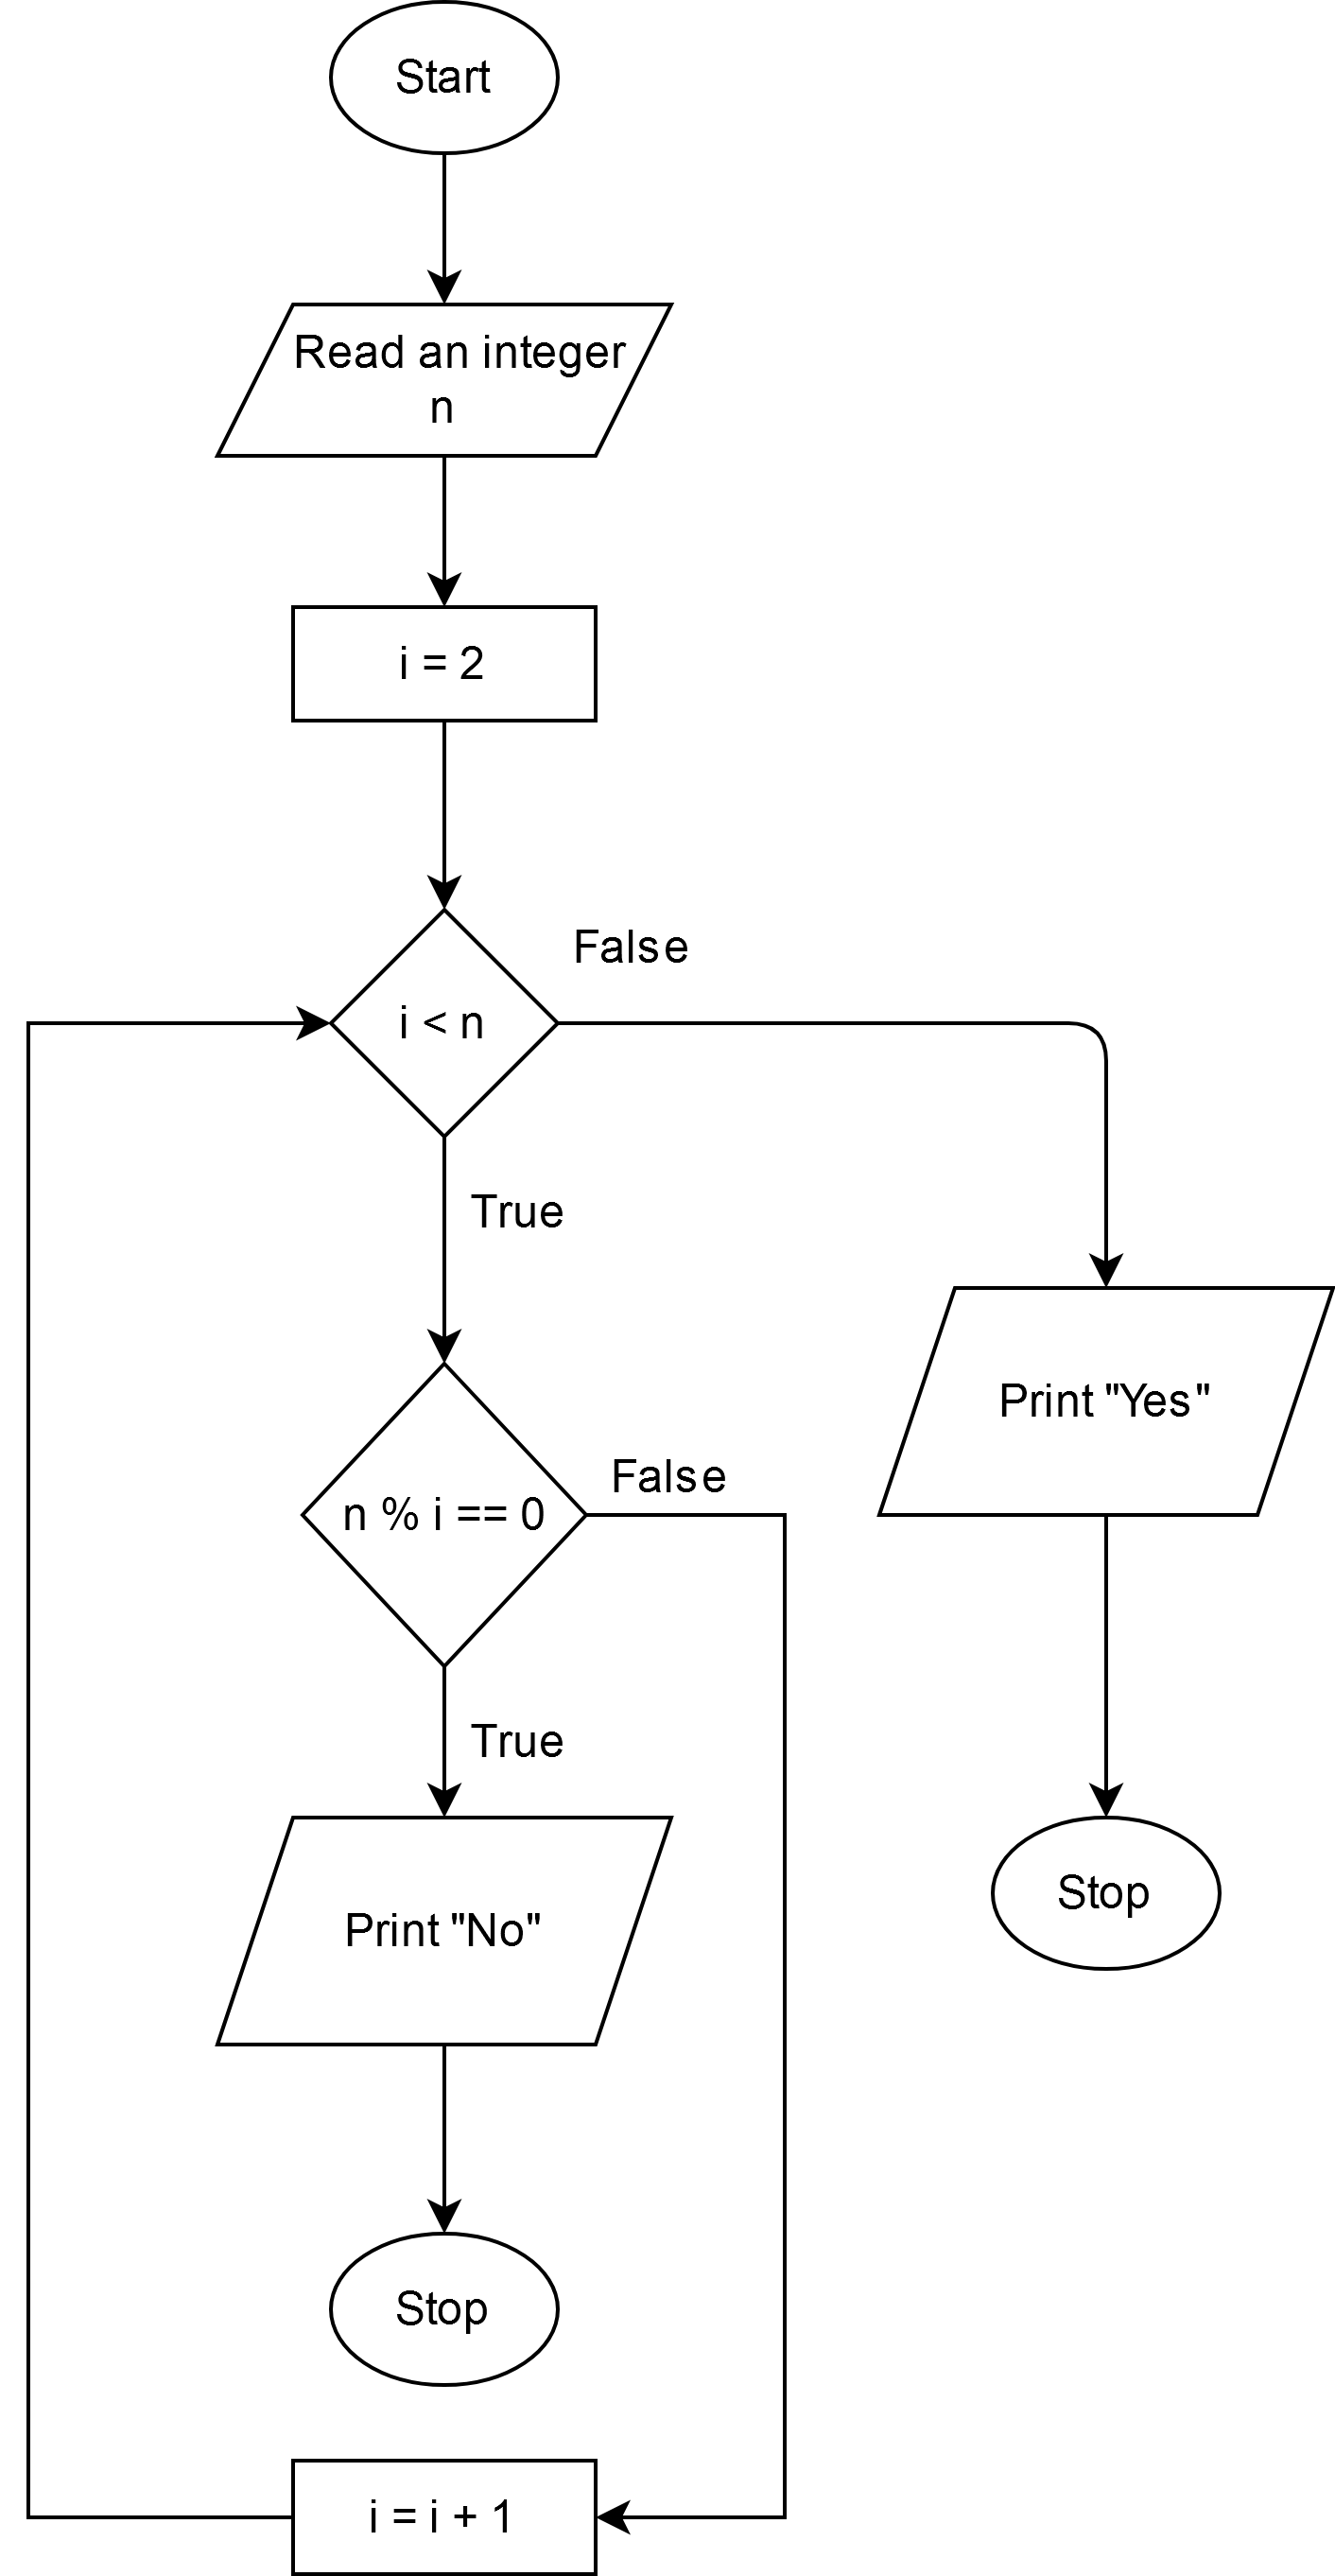
\includegraphics[width=0.5\textwidth]{Q2.png}
        \caption{Sample flowchart for Q2}
        \label{Q2}
    \end{figure}
    
    \clearpage


\begin{flushleft}

    \textbf{Q 3. } Draw a flowchart that takes a positive integer as input and 
    displays the number of divisors of the given number.
    
    \end{flushleft}
    
    \begin{flushleft}
    
    \textbf{Ans. } We can modify the solution to the previous question by 
    starting from 1 and maintaining the count of divisors in a separate variable 
    and updating it everytime a new divisor is found, instead of halting when the 
    first divisor is found. This is shown in Fig \ref{Q3}.

    We can optimise this by iterating only until $\sqrt{n}$ and adding 2 whenever
    the number is strictly less than $\sqrt{n}$. If the number is exactly $\sqrt{n}$
    then we should add 1. This optimisation is not required.
    
    \end{flushleft}
    
    \begin{flushleft}
    
    \textbf{Grading. } If the output of the flowchart is correct then 2, if there are 
    any errors, but the overall intent is correct then 1, otherwise 0.
    
    \end{flushleft}
    
    \begin{figure}[ht]
        \centering
        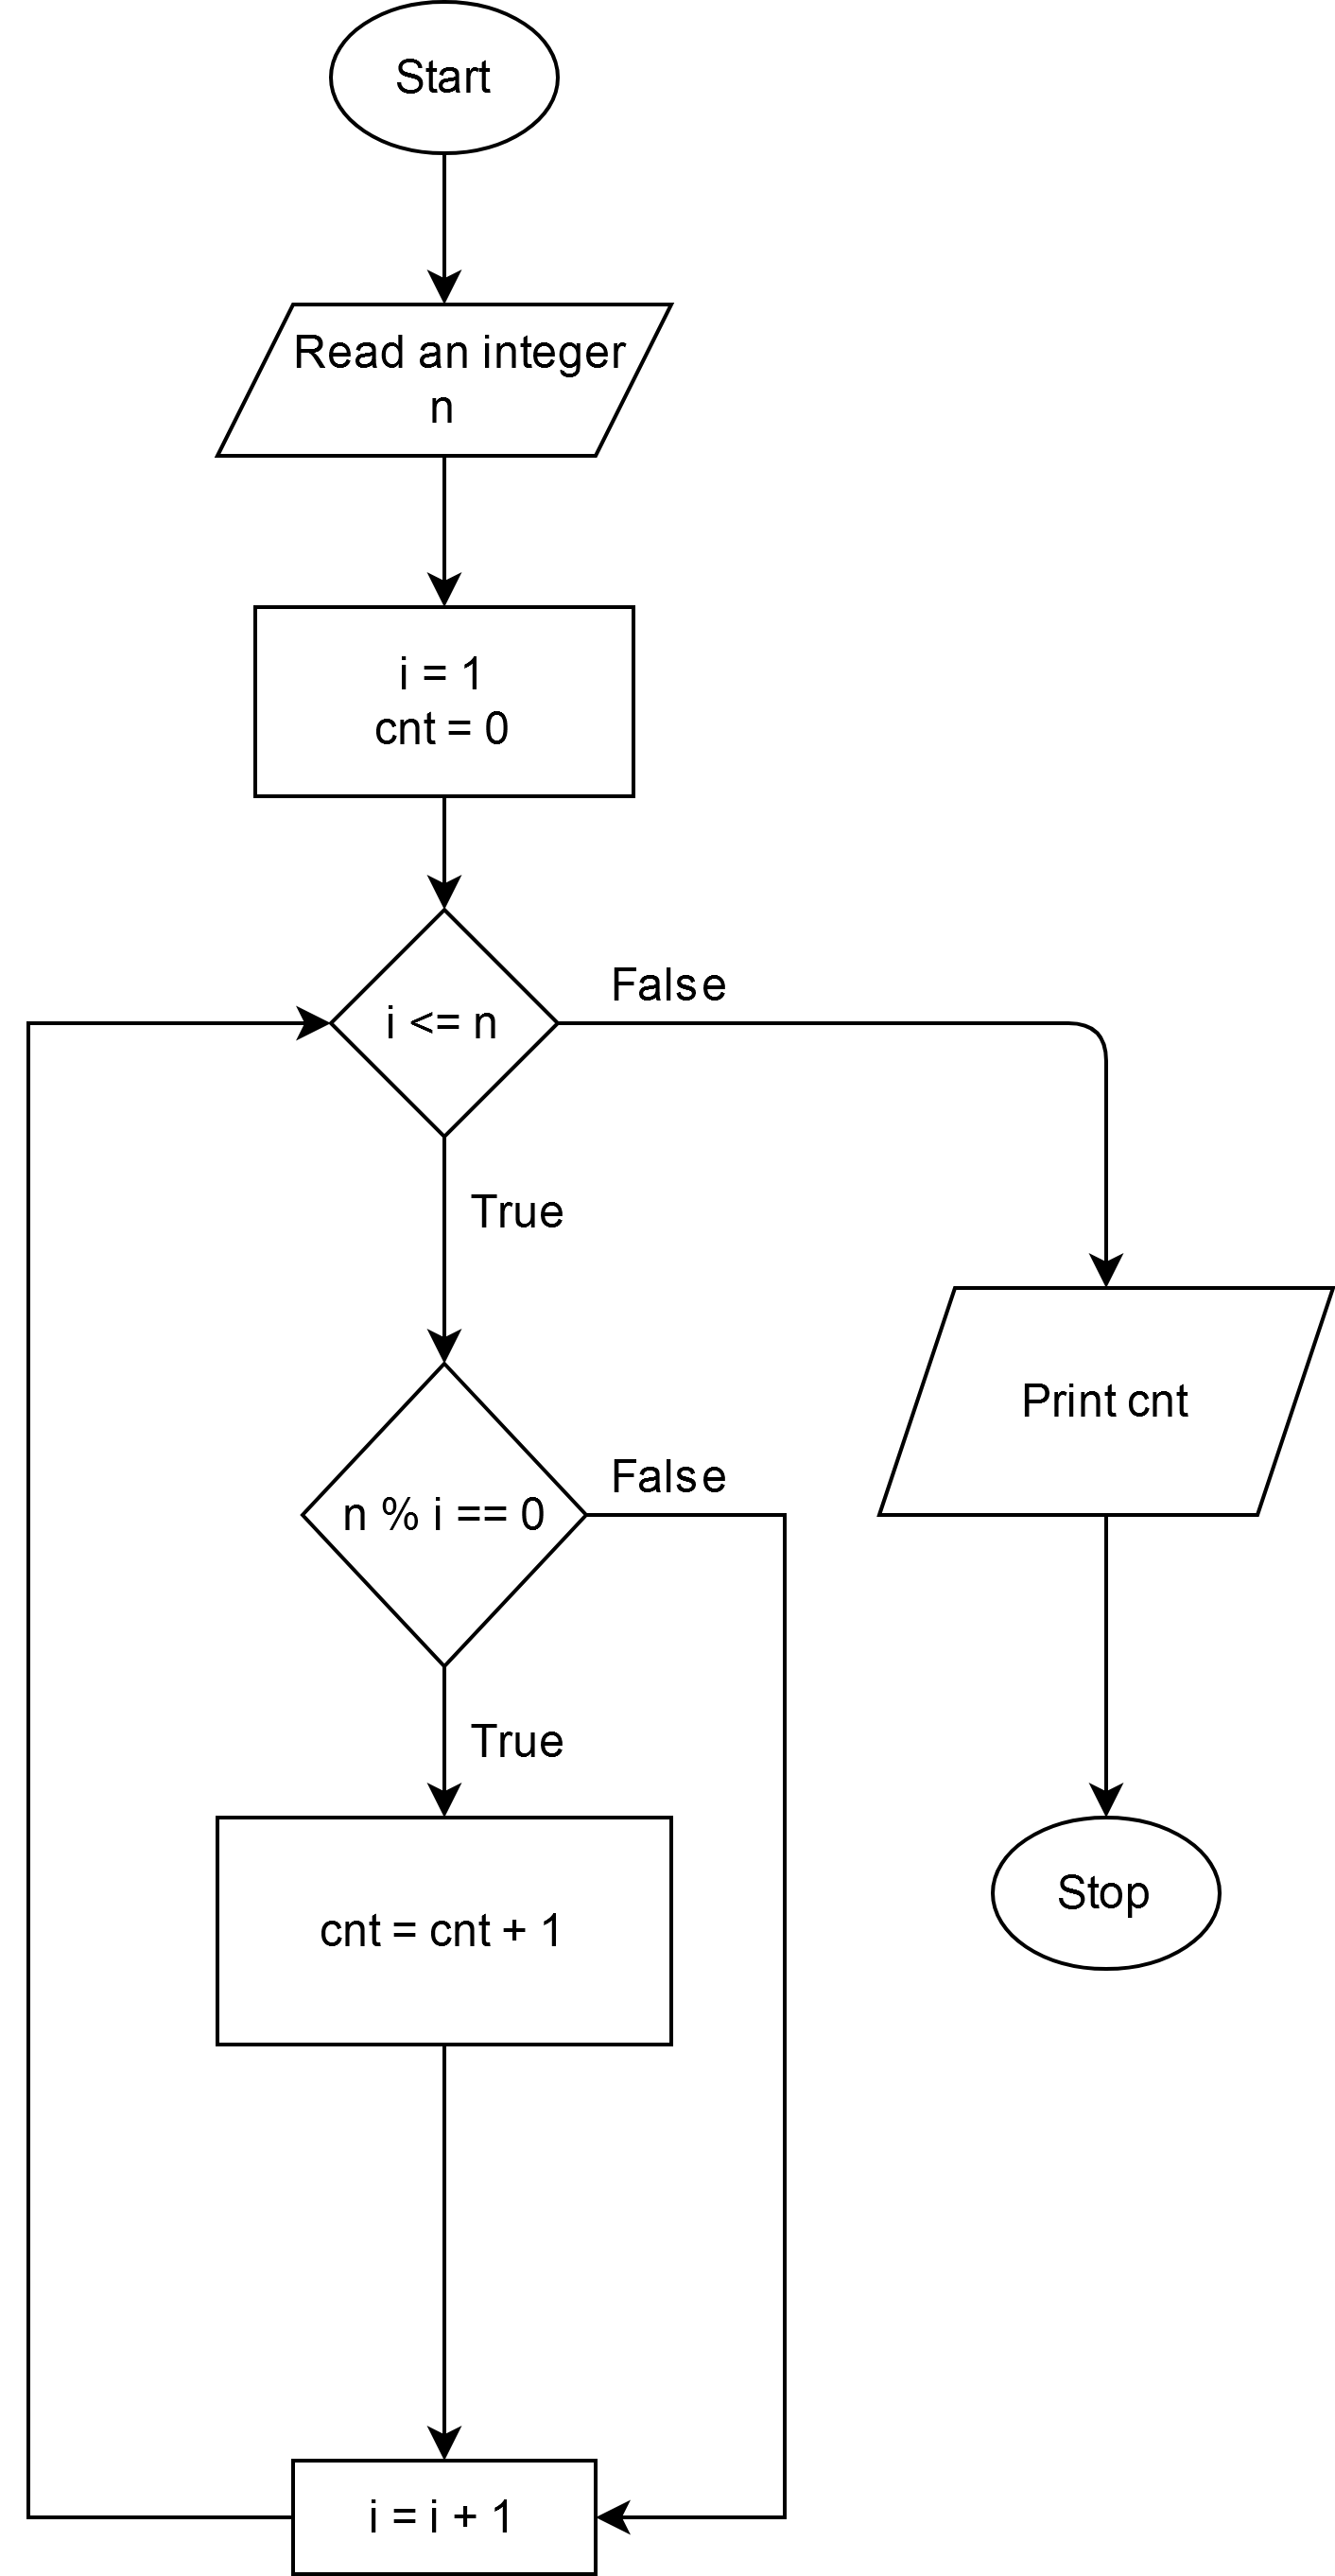
\includegraphics[width=0.5\textwidth]{Q3.png}
        \caption{Sample flowchart for Q3}
        \label{Q3}
    \end{figure}
    
    \clearpage


\begin{flushleft}
    \textbf{Q 4. } Draw a flowchart that takes as input the following
    \begin{itemize}
        \item A positive integer “n”, the number of students in the class
        \item A positive integer “m”, the number of the subjects
              taught
    \end{itemize}

    and for \textbf{each} student

    \begin{itemize}
        \item "m" integers, the marks of the student in each subject 
    \end{itemize}

    and displays the average marks of \textbf{each} student. (Assume that marks
    are given out of 100).
    
    \end{flushleft}
    
    \begin{flushleft}
    
    \textbf{Ans. } While taking input marks of a student, we maintain the sum 
    of the marks obtained from input so far, and finally print the sum / m at the 
    end, before obtaining input for the next student. This is shown in Fig \ref{Q4}.
    
    \end{flushleft}
    
    \begin{flushleft}
    
    \textbf{Grading. } If the output of the flowchart is correct then 2, if there are 
    errors but the overall intent is correct then 1, otherwise 0.
    
\end{flushleft}
    
    \begin{figure}[ht]
        \centering
        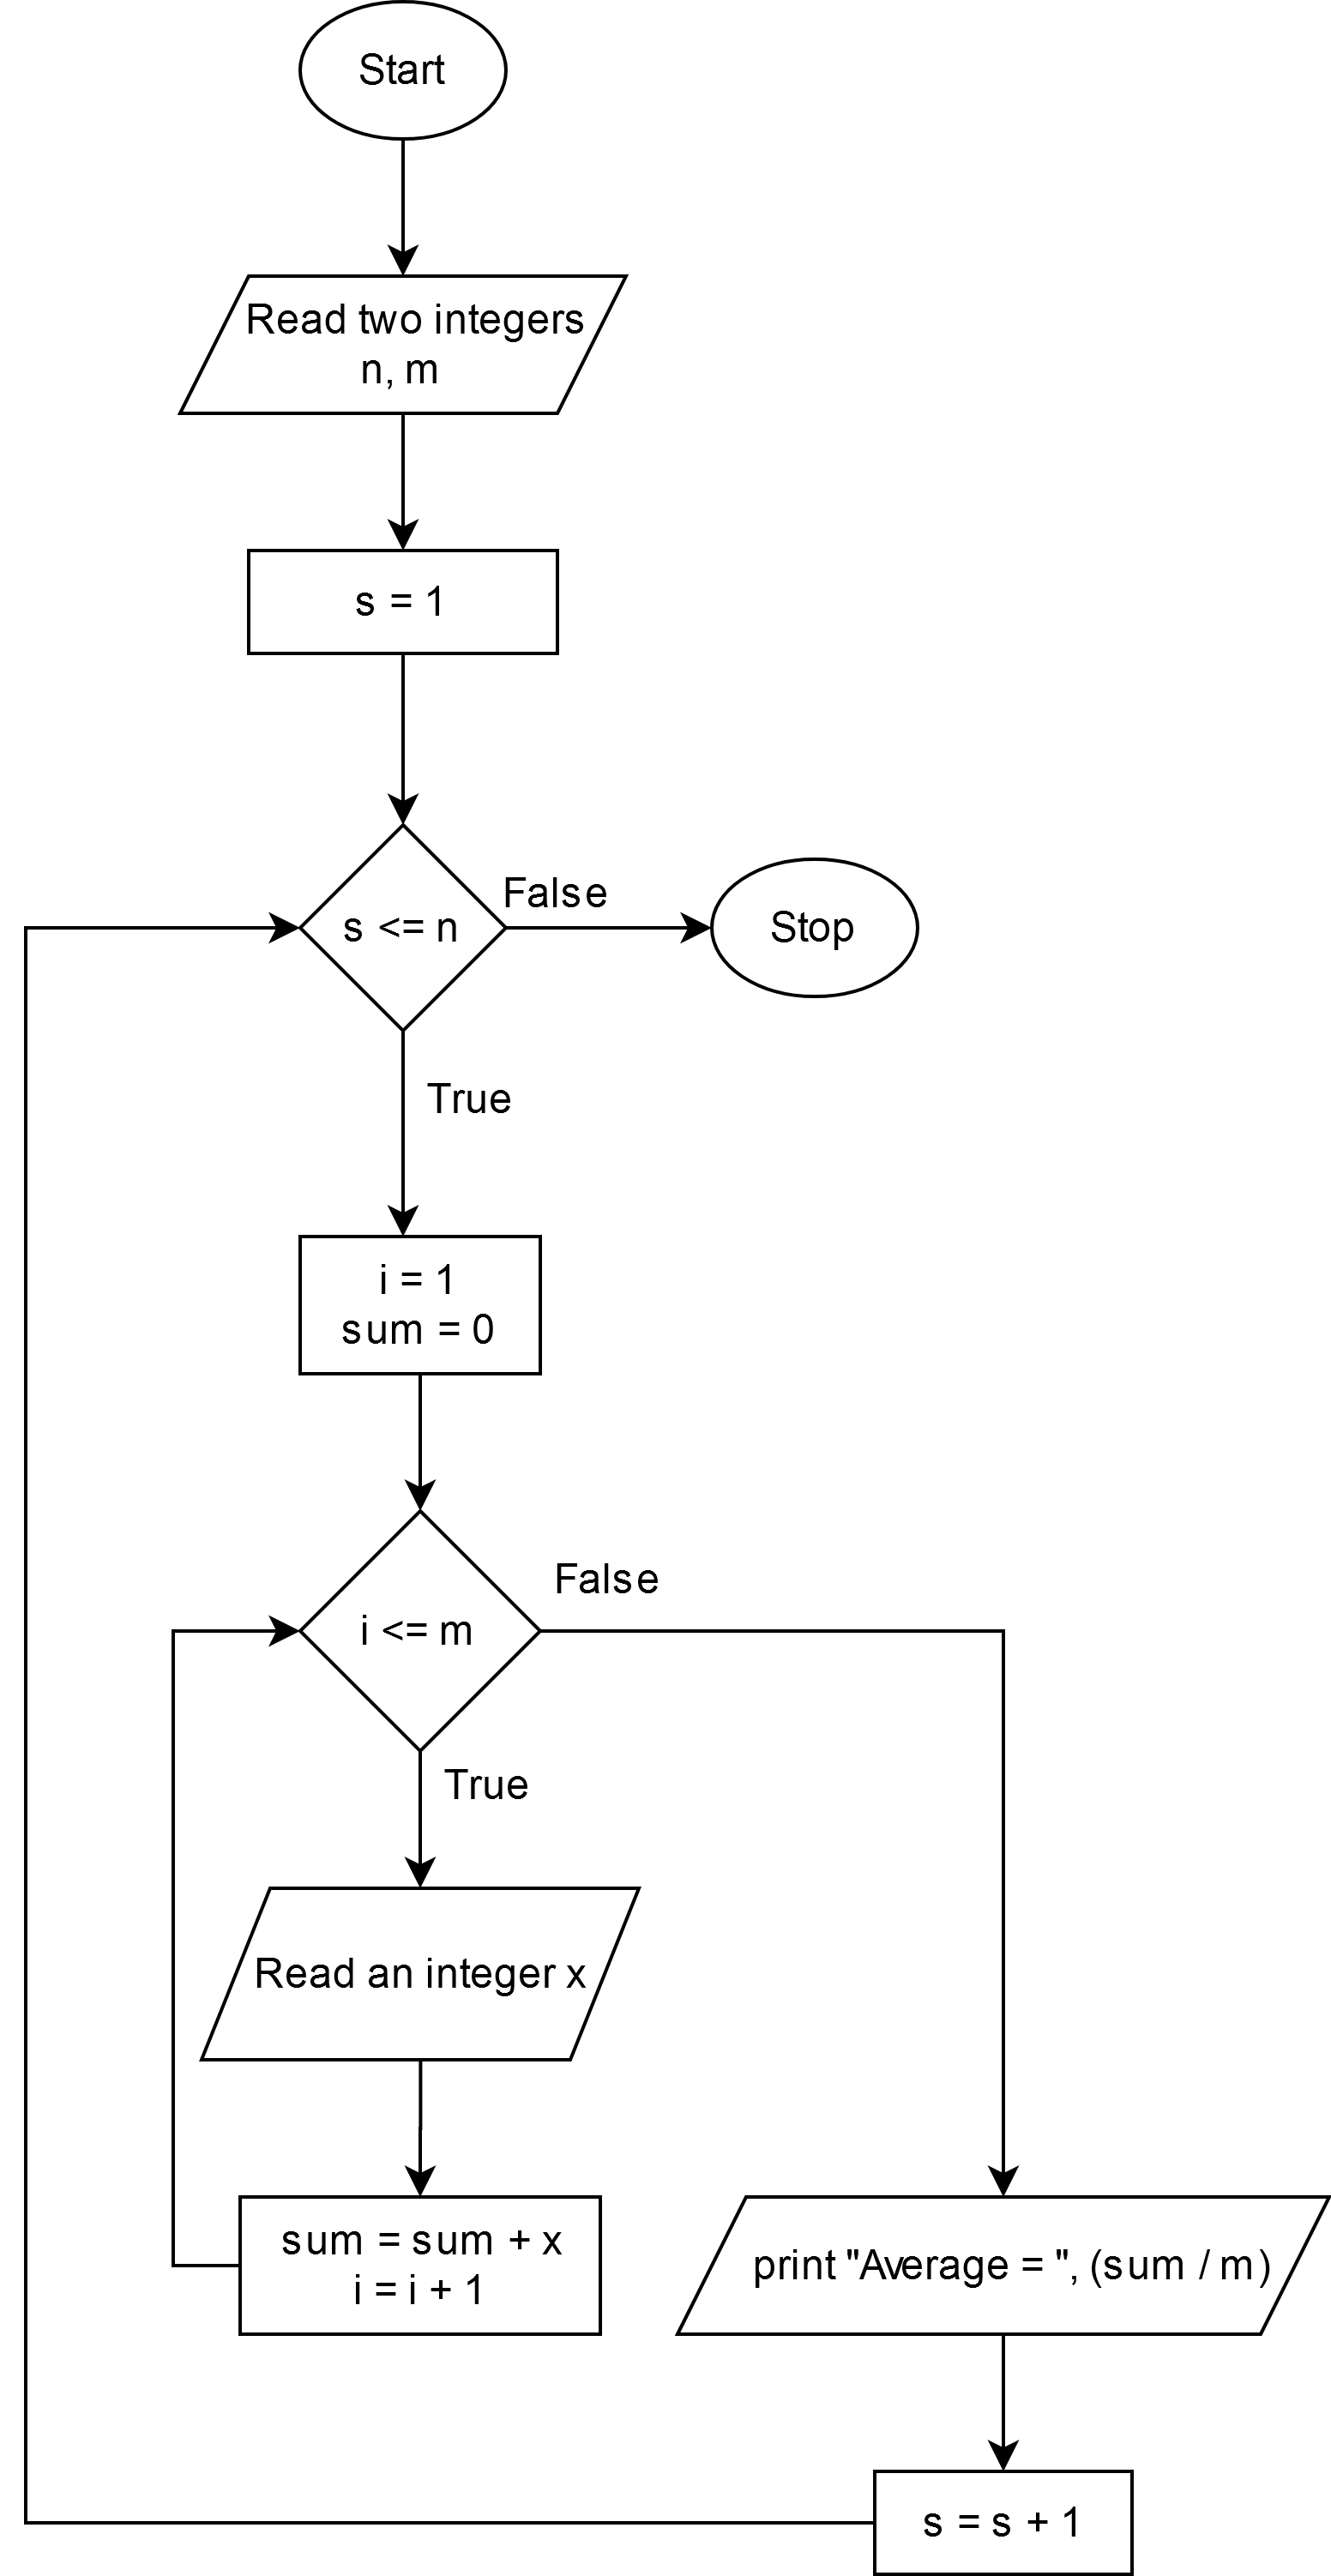
\includegraphics[width=0.5\textwidth]{Q4.png}
        \caption{Sample flowchart for Q4}
        \label{Q4}
    \end{figure}
    
    \clearpage


\begin{flushleft}
    \textbf{Q 5. } Draw a flowchart that takes as input a positive integer “N” 
    and prints all the elements of the sequence 1, 2, 4, 8,... which are less 
    than or equal to N. 
    How many numbers are printed if N = 1048575?
    
    \end{flushleft}
    
    \begin{flushleft}
    
    \textbf{Ans. } We can generate all powers of two and stop whenever the result
    is greater than N. Suppose the number of elements is $x$, then $2^x \leq N$,
    therefore $x \leq \log_2{N}$, for N = 1048575, $x \leq 19$, so a total of $20$
    numbers are printed (from $x = 0$ to $x = 19$).

    The sample flowchart is given in Fig \ref{Q5}.
    
    \end{flushleft}
    
    \begin{flushleft}
    
    \textbf{Grading. } If the correct answer (20) is mentioned and flowchart is
    correct then 2. If either answer (20) is wrong or there are errors in the 
    flowchart then 1, otherwise 0. Not printing spaces, is not considered as an 
    error.
    
    \end{flushleft}
    
    \begin{figure}[ht]
        \centering
        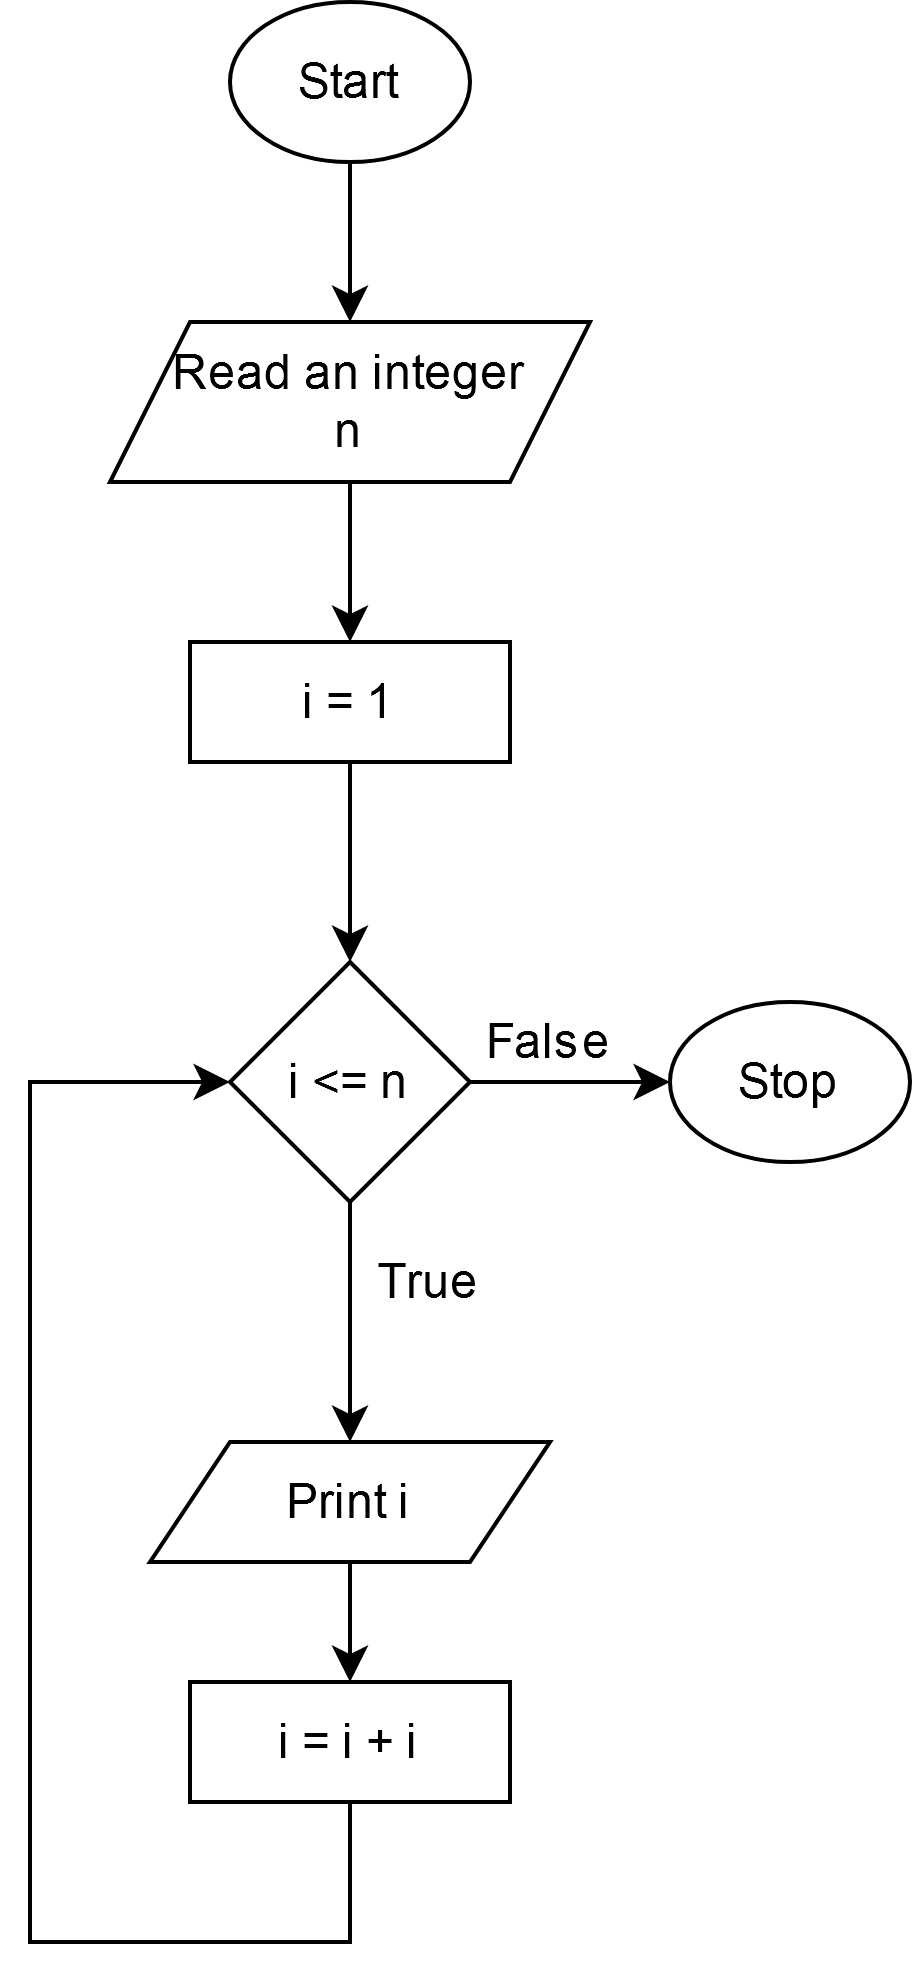
\includegraphics[width=0.5\textwidth]{Q5.png}
        \caption{Sample flowchart for Q5}
        \label{Q5}
    \end{figure}
    
    \clearpage


\begin{flushleft}
    \textbf{Q 6. } Draw a flowchart that takes a positive integer $n$ as input 
    and displays the largest integer $x$ such that $n$ is divisible by $2^x$.
    
    \end{flushleft}
    
    \begin{flushleft}
    
    \textbf{Ans. } If an integer is divisible by $2^x$ then it is also divisible
    by $2^{x-1}$. So we can iterate from $x=0$ and check for the first occurrence
    of a power of $2$, which does not divide $n$. Sample flowchart is shown in 
    Fig \ref{Q6}.
    
    \end{flushleft}
    
    \begin{flushleft}
    
    \textbf{Grading. } If the flowchart gives the correct output then 2, if there
    are errors but the overall intent is correct then 1, otherwise 0.
    
\end{flushleft}
    
    \begin{figure}[ht]
        \centering
        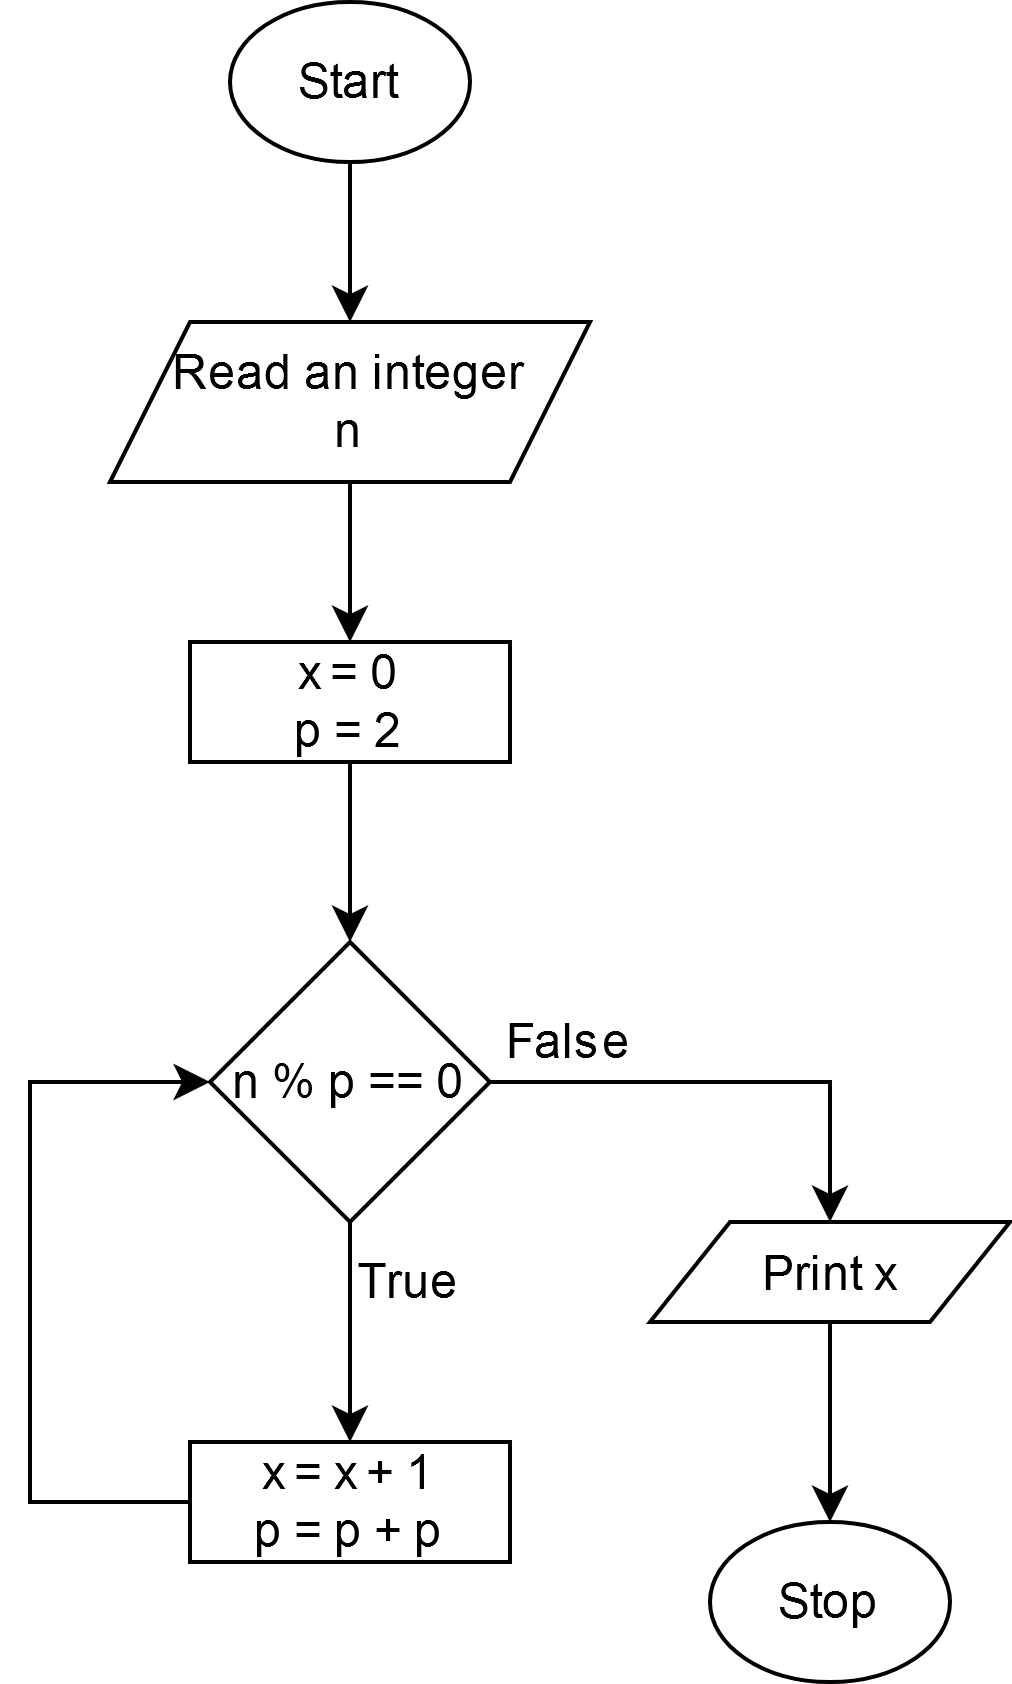
\includegraphics[width=0.5\textwidth]{Q6.png}
        \caption{Sample flowchart for Q6}
        \label{Q6}
    \end{figure}
    
\clearpage


\begin{flushleft}  

\textbf{Q 7. }  Draw a flowchart that takes a positive integer $n$ as input 
and displays $n$ in binary. For example, if $n = 9$ then display "1001".

\end{flushleft}

\begin{flushleft}

\textbf{Ans. } We first find the number of digits that we need to display. 
If the length is $x$ then $2^x$ is the smallest integer greater than $n$.
We can find $x$ in a similar manner to the previous question.

We then need to find the digits of $n$ from the most significant digit, so 
that we can print them in that order. 

We know that by definition the $(x-1)^{th}$ position will be "1" (otherwise 
length will not be $x$). To find the next set bit, lets remove this "1" from
the number $n$ (by subtracting $2^{x-1}$), and find the next power of $2$ which 
is less than or equal to the remaining number. That will be the next position 
where the binary representation has "1", and until then the digits will be "0".
This is shown in Fig \ref{Q7}.

\end{flushleft}

\begin{flushleft}

\textbf{Grading. } If the output of the flowchart is correct then 2, if there 
are minor errors then 1, otherwise 0.

\end{flushleft}

\begin{figure}[ht]
    \centering
    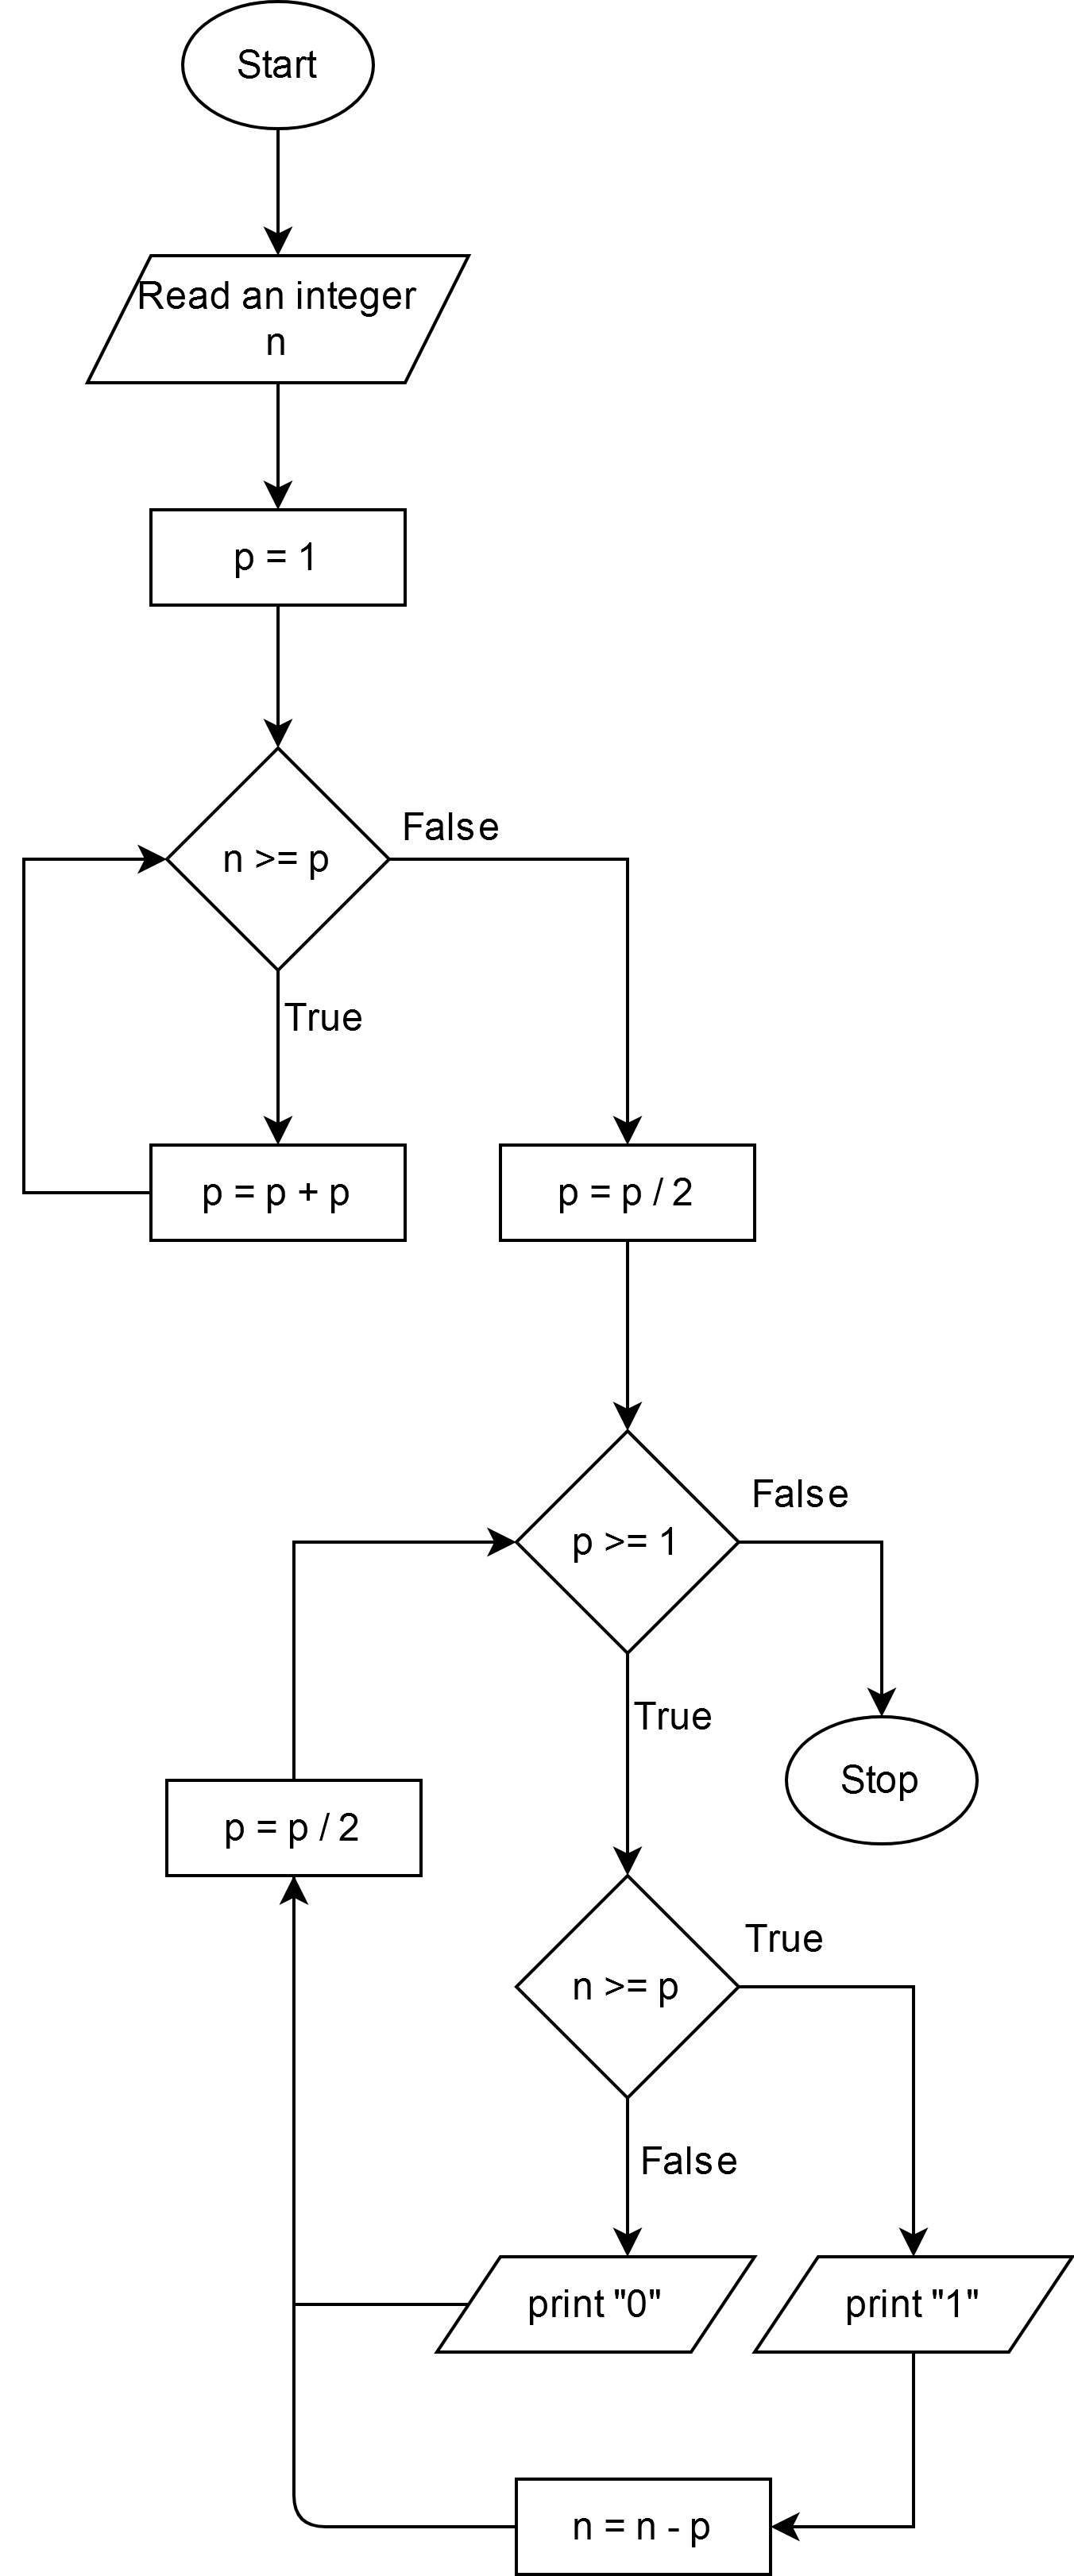
\includegraphics[width=0.5\textwidth]{Q7.png}
    \caption{Sample flowchart for Q7}
    \label{Q7}
\end{figure}

\clearpage


\begin{flushleft}

    \textbf{Q 8. } Draw a flowchart that takes a positive odd integer, height 
    of the pattern (height of the given example is 11) as input, and displays 
    the pattern (Fig \ref{Q8_fig}).

    \begin{figure}[ht]
        \centering
        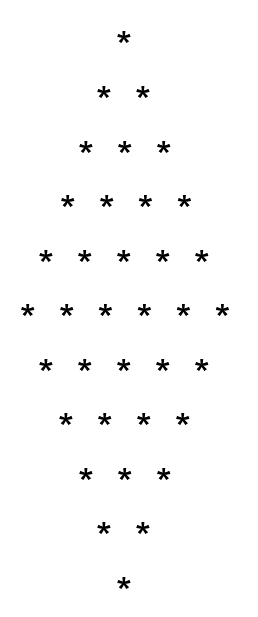
\includegraphics[width=0.3\textwidth]{Q8_fig.png}
        \caption{Pattern for flowchart}
        \label{Q8_fig}
    \end{figure}

    \end{flushleft}
    
    \begin{flushleft}
    
    \textbf{Ans. } As discussed in class, we can find out the number of
    spaces and "*"'s in each line and find a pattern for them.

    We print the top triangle part first and then the bottom part separately.

    Firstly we observe that there will be $\frac{h+1}{2}$ stars printed in the 
    middle row, and in row $y$, $\frac{h+1}{2} - y$ spaces should be printed
    before starting the "*"'s and $y$ stars should be printed with spaces between 
    them.

    For the last part, we repeat the same procedure for the top part, but 
    iterate from $y = h-1$ to $y = 1$. The flowchart is described in Fig \ref{Q8}.

    \end{flushleft}
    
    \begin{flushleft}
    
    \textbf{Grading. } Any correct flowchart that print a similar pattern is 
    considered correct. Even if spaces are not printed, but a nested loop with
    correct number of *'s in each row is printed, give 2. Statement's like 
    "*" * 5 for printing 5 consecutive "*"'s are also correct (although not 
    covered in class). If there are errors in the flowchart but method seems 
    correct then 1, otherwise 0.
    
    \end{flushleft}
    
    \begin{figure}[ht]
        \centering
        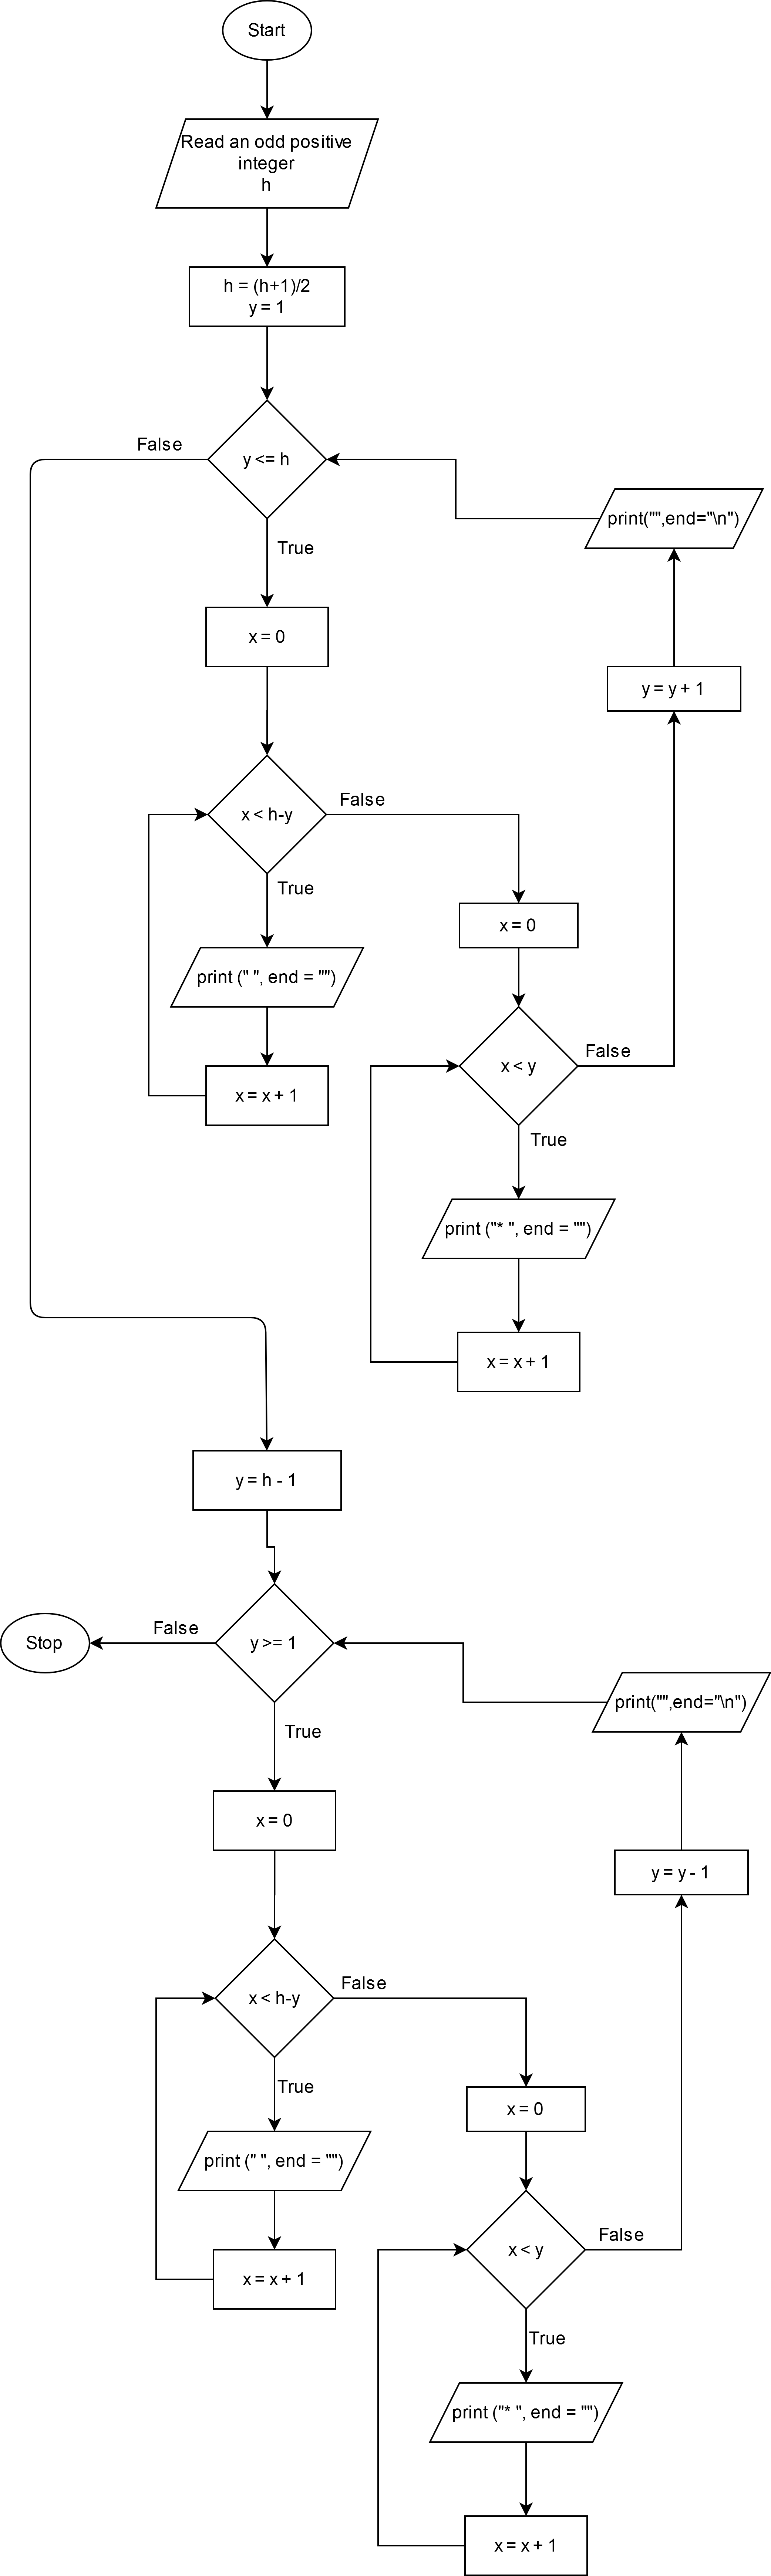
\includegraphics[width=0.35\textwidth]{Q8.png}
        \caption{Sample flowchart for Q8}
        \label{Q8}
    \end{figure}

\clearpage



\begin{flushleft}

    \textbf{Q 9. } Draw a flowchart that takes as input a positive number $n$ and 
    $n$ positive numbers, and displays the greatest common divisor of all the 
    numbers.

    For example:-  let n = 5 and numbers are - 3, 6, 12, 27, 33 so the 
    number that should be displayed is 3.  
    
    \end{flushleft}
    
    \begin{flushleft}
    
    \textbf{Ans. } Let's maintain a variable $g$ to be the gcd of all the numbers
    taken as input so far. Note that $g$ can only decrease when more numbers are 
    added. The second observation is that all common divisors will be divisors 
    of $g$.

    For the first number, $g$ will be equal to the number taken as input.
    For the subsequent numbers if there's a change in the gcd, it will be a 
    factor of the number already obtained so far. 

    So we can iterate from $g$ to $1$ and find the first number which is both 
    a factor a $g$ and the number read from input. 

    In this way we can get the gcd of all the numbers. 
    Flowchart is shown in Fig \ref{Q9}.

    A more efficient way is to use Euclid's algorithm for gcd, which will 
    require less operations, however it was not required.
    
    \end{flushleft}
    
    \begin{flushleft}
    
    \textbf{Grading. } Any valid method for obtaining the gcd correctly for 
    $n$ numbers is given 2. If there are errors in the flowchart then 1. 
    If there are any logical errors then 0.
    
    \end{flushleft}
    
    \begin{figure}[ht]
        \centering
        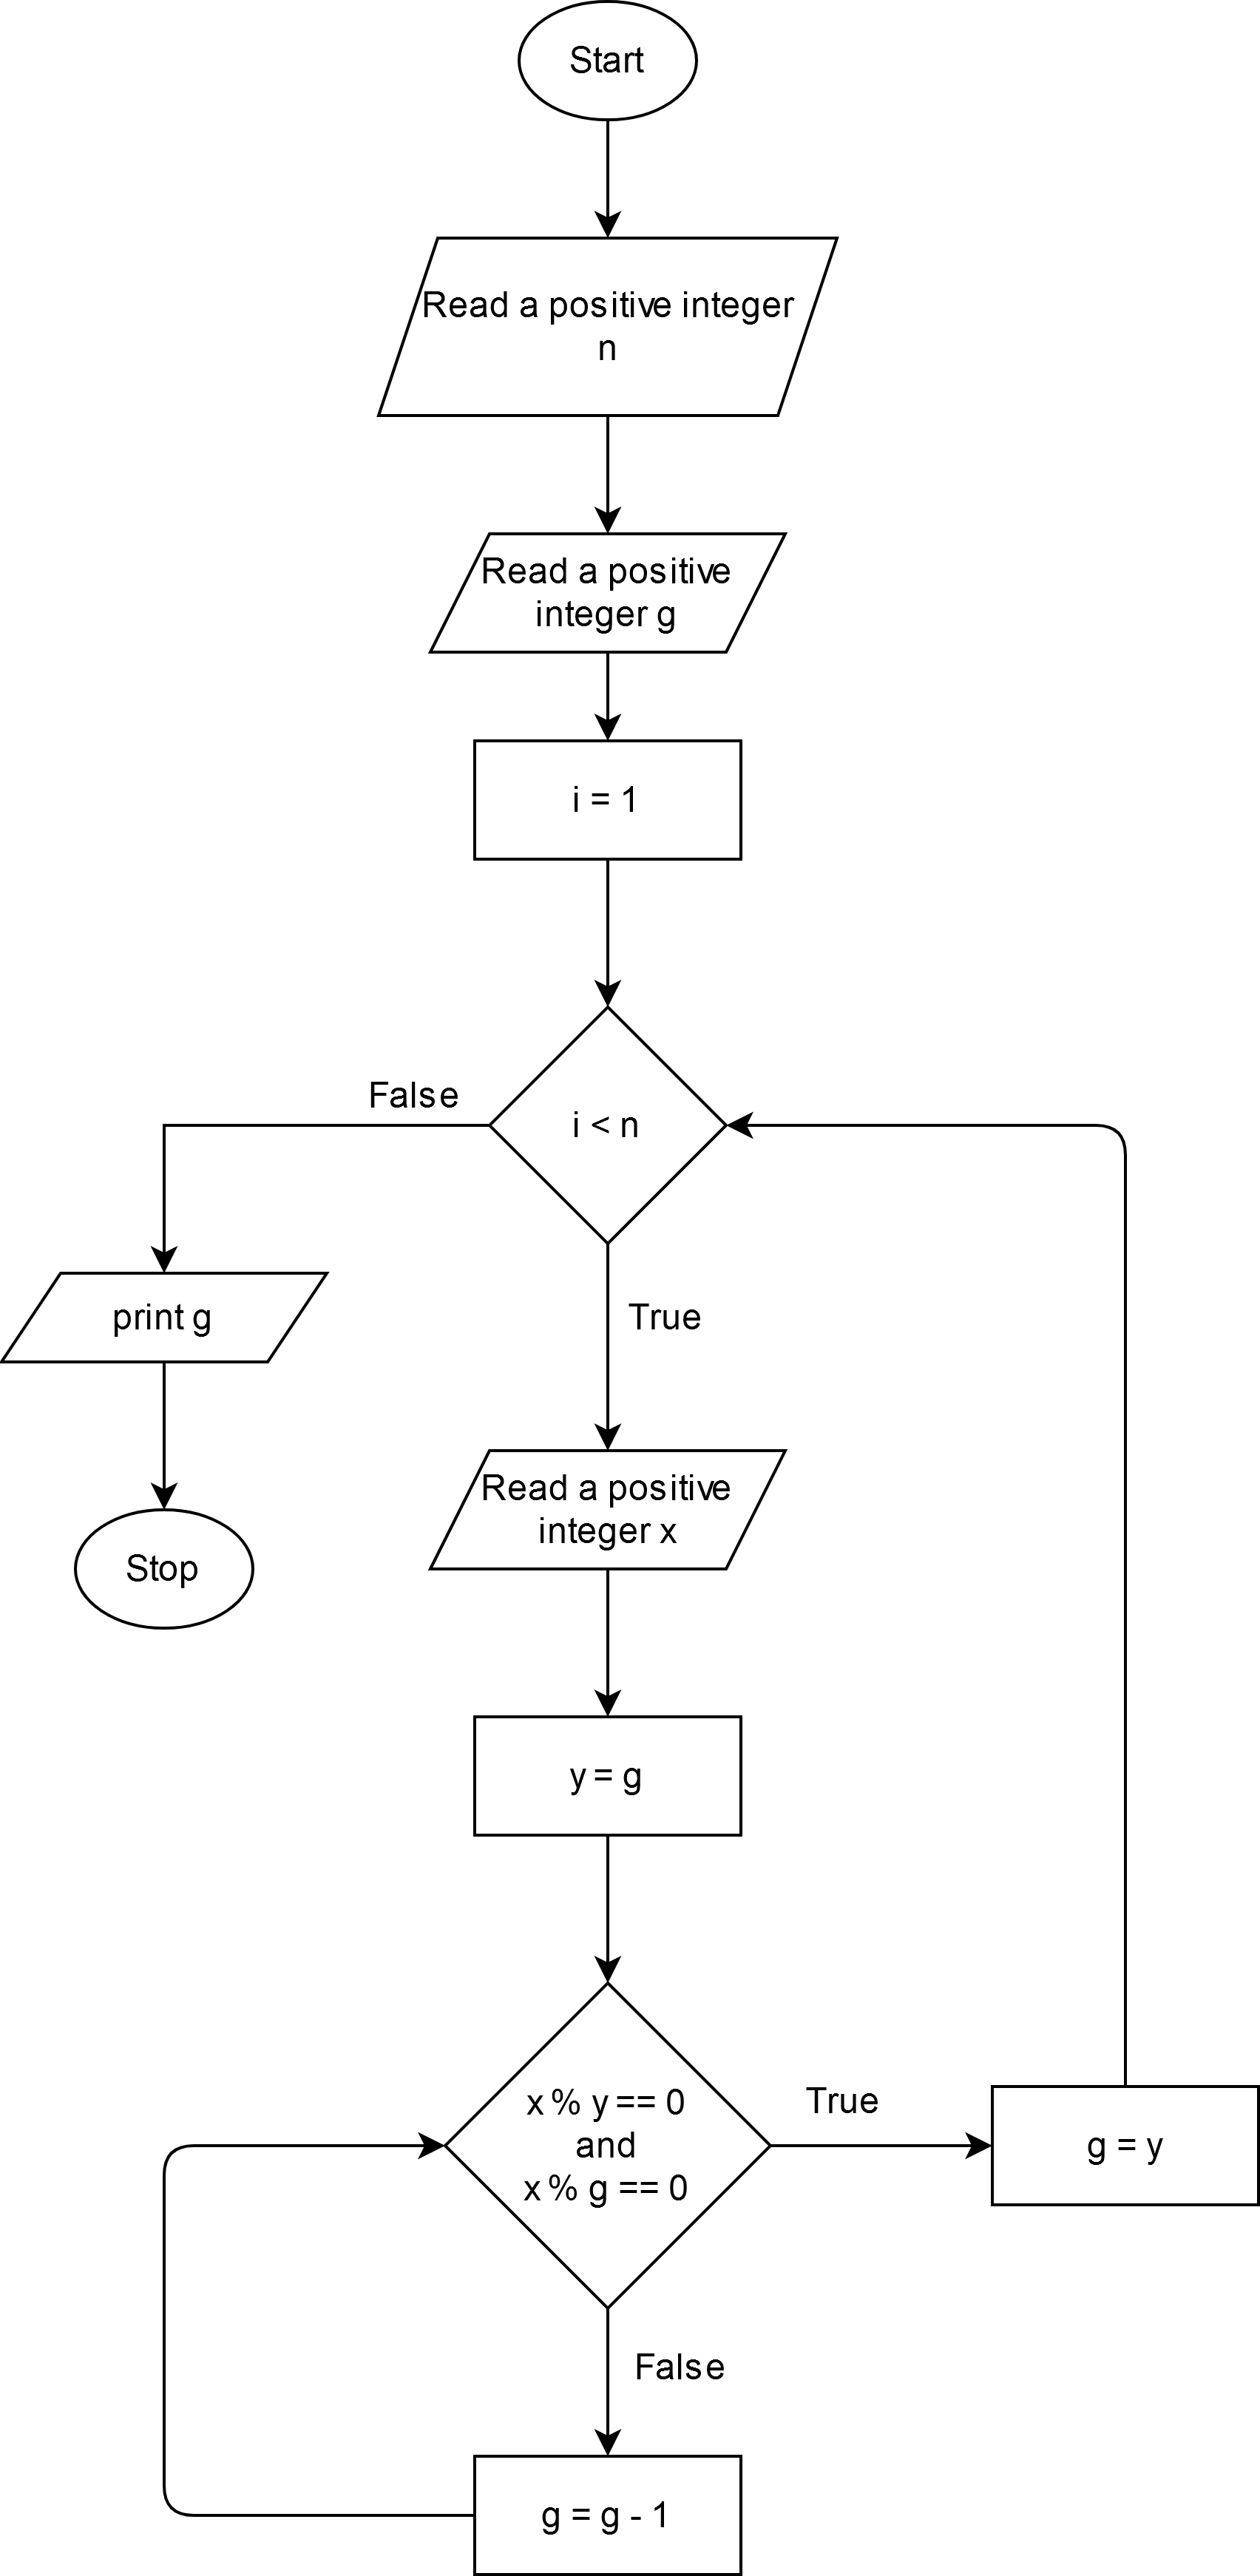
\includegraphics[width=0.5\textwidth]{Q9.png}
        \caption{Sample flowchart for Q9}
        \label{Q9}
    \end{figure}
    
    \clearpage

    
\begin{flushleft}

    \textbf{Q 10. } Draw a flowchart that takes a positive number $h$, 
    the height (height of the given example (Fig \ref{Q10_fig}) is 5 (starting 
    from 0)), as input and displays 
    \href{https://en.wikipedia.org/wiki/Pascal%27s_triangle}{Pascal's triangle} 
    up to height $h$.
    Note: Print two spaces between two consecutive numbers.

    \begin{figure}[ht]
        \centering
        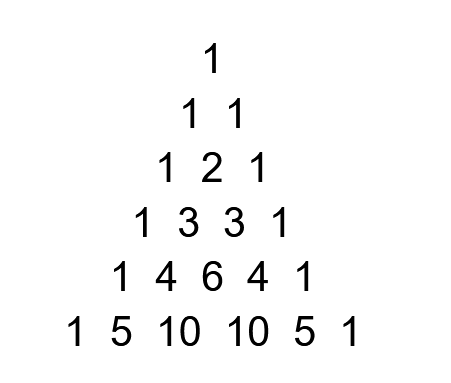
\includegraphics[width=0.3\textwidth]{Q10_fig.png}
        \caption{Example for Q10}
        \label{Q10_fig}
    \end{figure}
    
    
    \end{flushleft}
    
    \begin{flushleft}
    
    \textbf{Ans. } Similar to Q8, we have two nested loops, one for printing 
    each line and one to go to subsequent lines.

    We can make use of the fact that the $r^{th}$ (starting from $0$) number 
    on the $n^{th}$ line will be $\binom{n}{r}$ and the formula 
    $\binom{n}{r+1} = \frac{\binom{n}{r} * (n-r)}{r+1}$ to get the 
    answer. The flowchart is given in Fig \ref{Q10}.

    
    \end{flushleft}
    
    \begin{flushleft}
    
    \textbf{Grading. } If the output of the flowchart is correct then 2. 
    If there are functions used for factorial, or binomial coefficient, and 
    flowcharts for those functions are written separately, the answer is 
    considered correct (2). However if functions are used and flowcharts for them 
    are not given then give 1. If output is not correct then 0.
    
    \end{flushleft}
    
    \begin{figure}[ht]
        \centering
        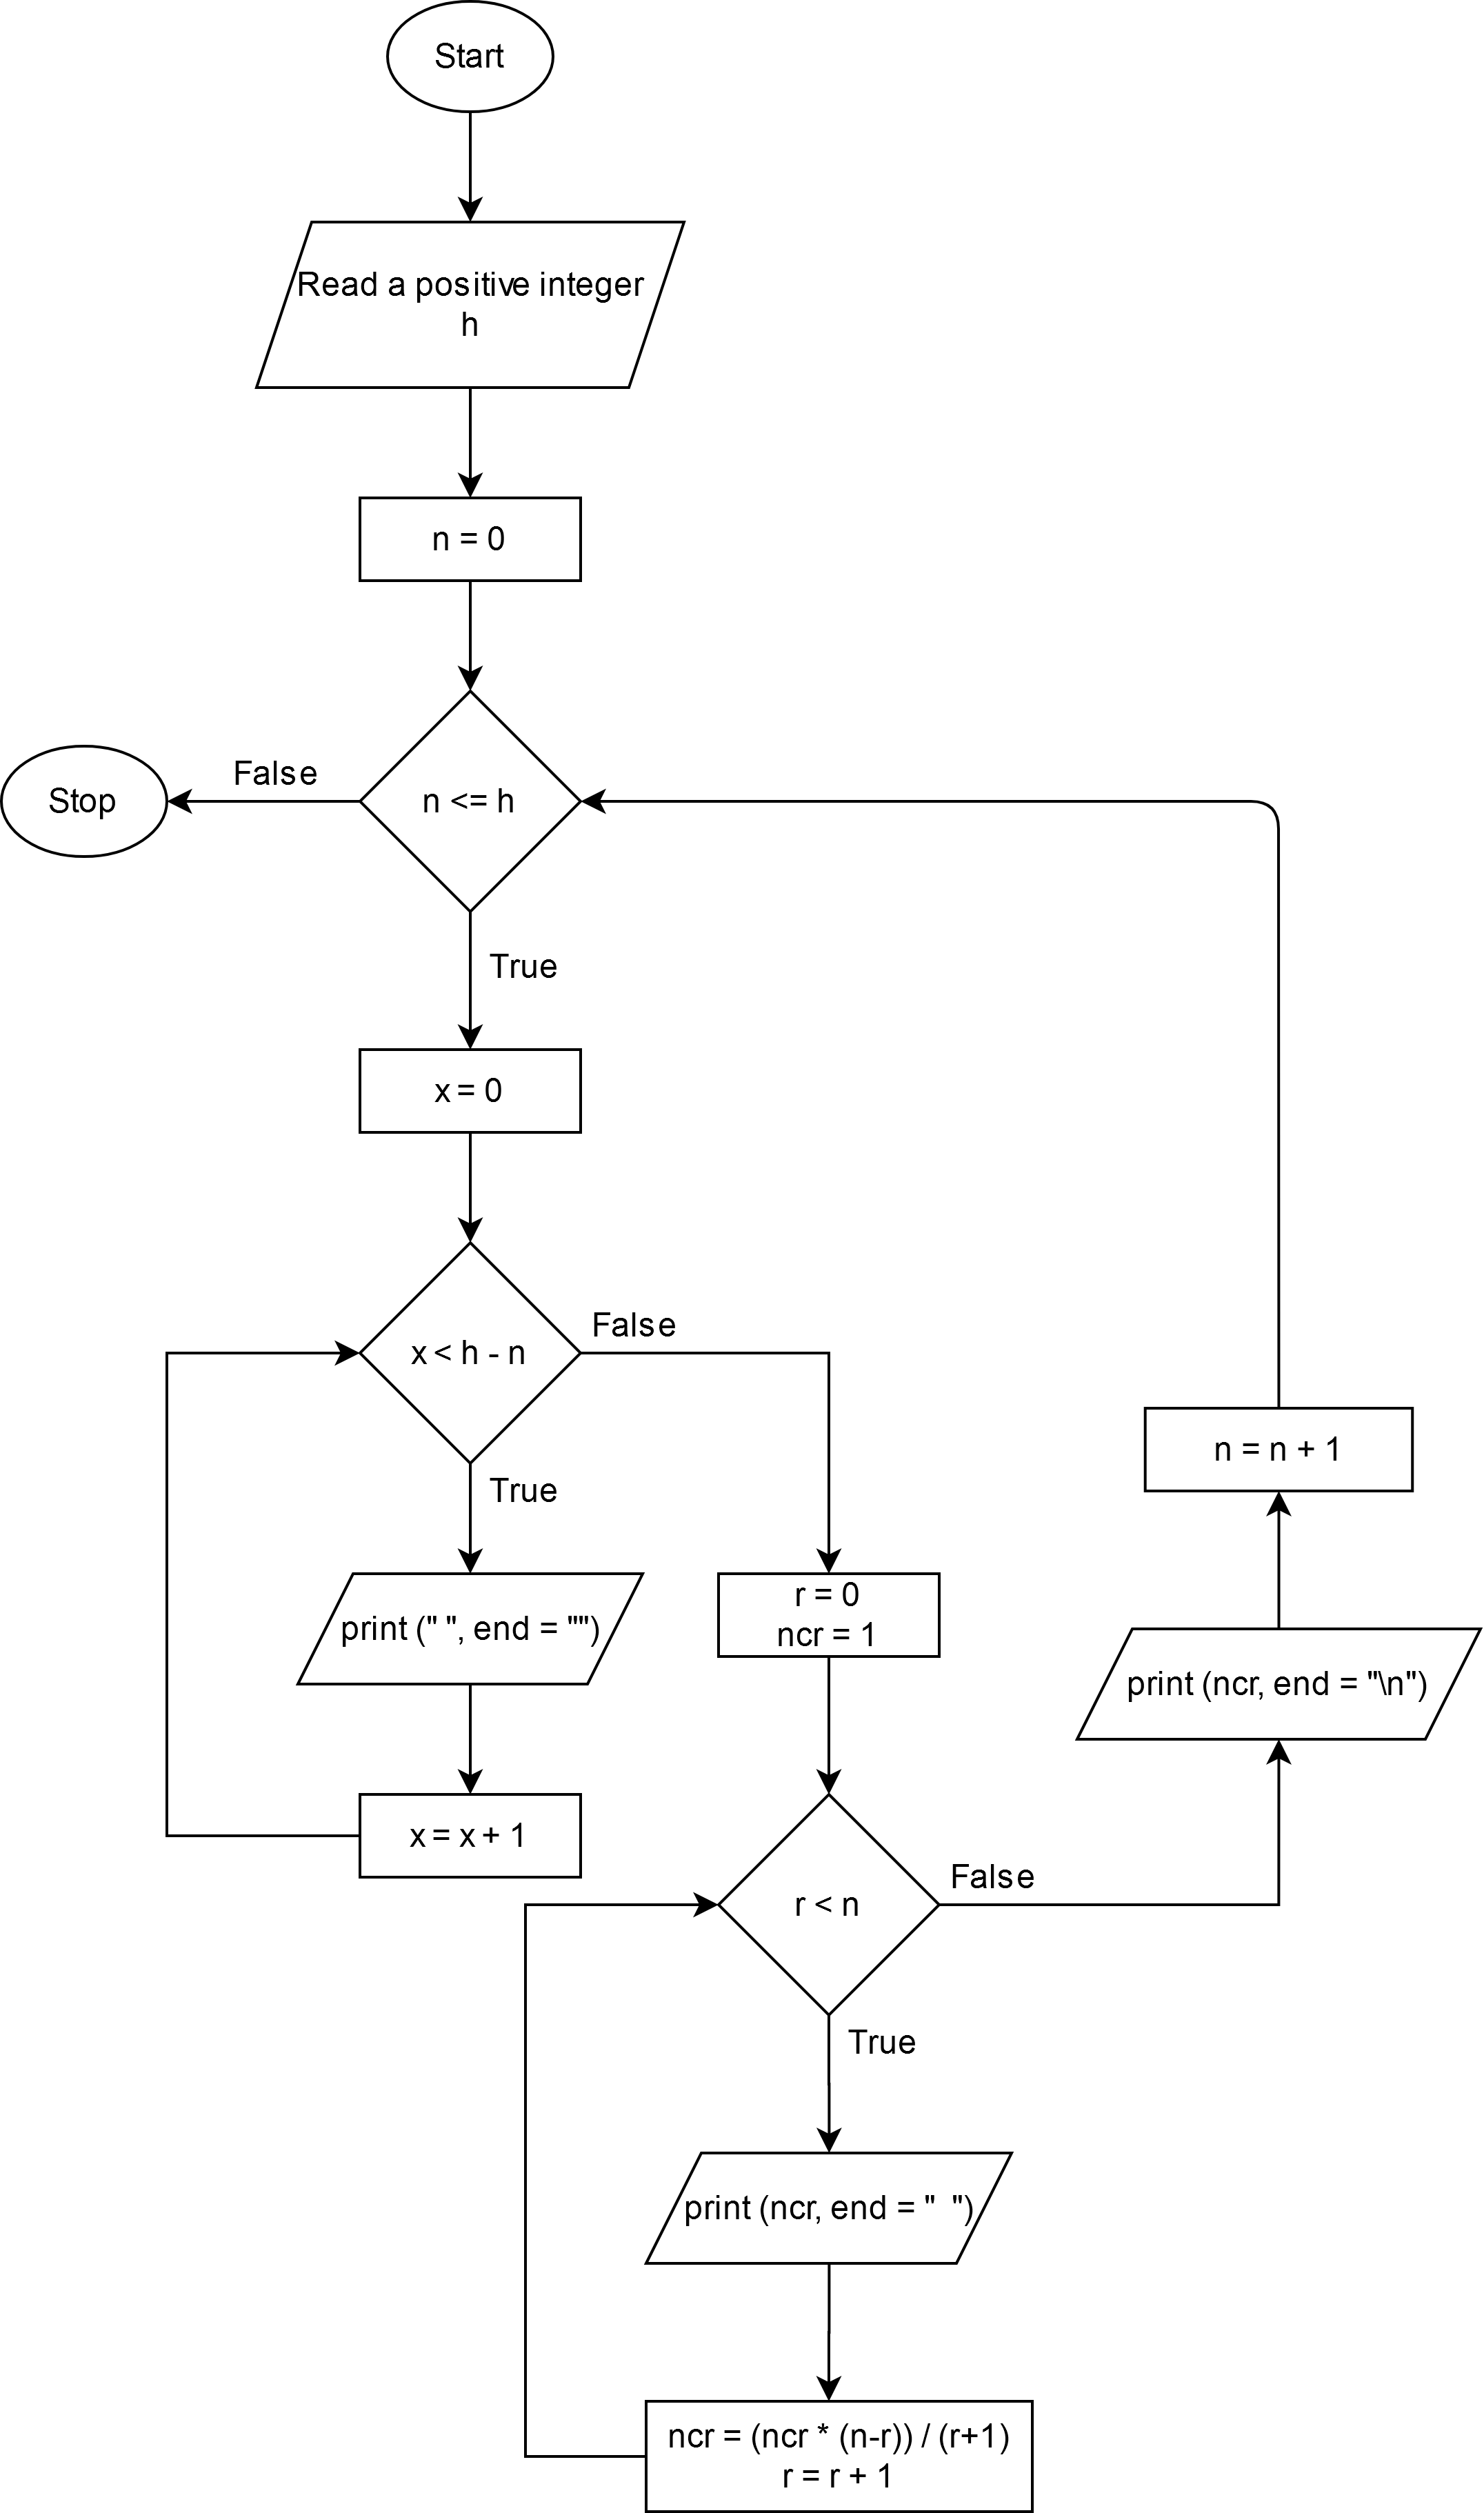
\includegraphics[width=0.5\textwidth]{Q10.png}
        \caption{Sample flowchart for Q10}
        \label{Q10}
    \end{figure}
    
    \clearpage

\comment{

\begin{flushleft}

\textbf{Q 1. } 

\end{flushleft}

\begin{flushleft}

\textbf{Ans. } 

\end{flushleft}

\begin{flushleft}

\textbf{Grading. }

\end{flushleft}

\begin{figure}[ht]
    \centering
    \includegraphics[width=0.5\textwidth]{}
    \caption{Sample flowchart for Q}
    \label{Q}
\end{figure}

\clearpage
}

\end{document}